% !TeX spellcheck = en_GB

\documentclass{beamer}

\usetheme{Warsaw}             % Falls Ihnen das Layout nicht gef�llt, k�nnen Sie hier
                              % auch andere Themes w�hlen. Ein Verzeichnis der m�glichen 
                              % Themes finden Sie im Kapitel 15 des beameruserguide.


\setbeamertemplate{footline}[frame number] %Seitenzahlen

\usepackage[utf8]{inputenc} % um Umlaute direkt eingeben zu
\usepackage[english]{babel}
\usepackage{amsmath}
\usepackage{amsfonts}
\usepackage{amssymb}
\usepackage{graphicx}
\usepackage{tikz}
\usepackage{stmaryrd} % for llbracket
\usepackage{algorithm} %for algorithms
\usepackage{algpseudocode} %for algorithms
%\usepackage{caption}
\usepackage{subcaption} %for subfigure
\usepackage[3D]{movie15} %for interactve 3d plot 

\usepackage{wrapfig} % for using wrapfigure

\usepackage{bigdelim}
\usepackage{caption}
\usepackage{subcaption}
\usepackage{ltxtable}
\usepackage{float}
%\usepackage{pgfplotstable, booktabs} %to generate tables from data files


\usepackage{../Arbeit/makros}
\usepackage{todo}

\makeatletter
% Detect mode. mathpalette is used to detect the used math style
\newcommand<>\Alt[2]{%
    \begingroup
    \ifmmode
        \expandafter\mathpalette
        \expandafter\math@Alt
    \else
        \expandafter\make@Alt
    \fi
    {{#1}{#2}{#3}}%
    \endgroup
}

% Un-brace the second argument (required because \mathpalette reads the three arguments as one
\newcommand\math@Alt[2]{\math@@Alt{#1}#2}

% Set the two arguments in boxes. The math style is given by #1. \m@th sets \mathsurround to 0.
\newcommand\math@@Alt[3]{%
    \setbox\z@ \hbox{$\m@th #1{#2}$}%
    \setbox\@ne\hbox{$\m@th #1{#3}$}%
    \@Alt
}

% Un-brace the argument
\newcommand\make@Alt[1]{\make@@Alt#1}

% Set the two arguments into normal boxes
\newcommand\make@@Alt[2]{%
    \sbox\z@ {#1}%
    \sbox\@ne{#2}%
    \@Alt
}

% Place one of the two boxes using \rlap and place a \phantom box with the maximum of the two boxes
\newcommand\@Alt[1]{%
    \alt#1%
        {\rlap{\usebox0}}%
        {\rlap{\usebox1}}%
    \setbox\tw@\null
    \ht\tw@\ifnum\ht\z@>\ht\@ne\ht\z@\else\ht\@ne\fi
    \dp\tw@\ifnum\dp\z@>\dp\@ne\dp\z@\else\dp\@ne\fi
    \wd\tw@\ifnum\wd\z@>\wd\@ne\wd\z@\else\wd\@ne\fi
    \box\tw@
}

\makeatother



\AtBeginSection[]{\frame<beamer>{\frametitle{Content} \tableofcontents[current]}}

%\titlehead{
\includegraphics[height=0.5cm]{../Arbeit/rwth.pdf} \hspace{1cm}
%
\includegraphics[height=0.5cm]{../Arbeit/IGPM_logo_klein.png}
%}

\subject{Master Thesis}
\title{Discontinuous Galerkin Methods for the \MA Equation}
\subtitle{\Large Discontinuous Galerkin Verfahren zur Lösung der Monge-Amp\`ere-Gleichung}
\author{Elisa Friebel} %\\ Matrikelnummer: 295932
\date{\today}
%\publishers{Gutachter: Prof. Dr. rer. nat. W. Dahmen\\ Prof. Dr. rer. nat. S. Noelle}
\date{11. Februar 2014 \\[.5\baselineskip] Seminarvortrag}

\begin{document}
\frame{\maketitle}

\section{\MA Equation}

\begin{frame}{The \MA Equation}
\begin{block}{\MA with Dirichlet Boundary Data}
 \begin{align*}
	 \mydet{D^2 u} &= f \textnormal{ in } \Omega \\ %\label{eq: MA eq}\\
	 u & = g \textnormal{ on } \partial \Omega, %\label{eq: MA equation dirilecht} 
 \end{align*}
 \end{block}
Applications areas of equation of \MA type
\begin{itemize}
	\item astrophysics
	\item differential geometry
	\item finance
	\item optimal transportation 
	\item optics
\end{itemize} 
\end{frame}

%\subsection{Existence and Uniqueness}
\begin{frame}{Existence}
	Let $F$ be the \MA operator, i.e. $F= \detHess{u} - f$
	\begin{itemize}
		\item F is fully nonlinear second order operator
		\item $F$ is elliptic for strictly convex functions $u$ and $f > 0$. %\cite{GT1983}
		\item existence of a classical solution depends on the regularity of the data and domain
		\item classical solutions are ambiguous
		\item no general weak formulation
	\end{itemize}
\end{frame}

\begin{frame}{Weak Solution Notion}
	\begin{block}{Viscosity Solution{\cite[Definition 1.1]{FGN2013}}}
		We call a strictly convex $u \in C^0(\Omega)$ a \emph{viscosity subsolution (supersolution)} of the \MA equation, if for every point $x_0 \in \Omega$ and function $\varphi \in C^2(\Omega)$ satisfying
		\[
		   u \leq \varphi \;(\geq \varphi) \text{ in }\Omega \text{  and  } u(x_0) = \varphi(x_0)
		\]		there holds
		\[
			F[\varphi](x_0) \leq 0 \;(\geq 0).%\mydet{D^2 \varphi(x_0)} - f \leq 0 (\geq 0).
		\]

\end{block}
	Viscosity solutions are unique.
	%u-\varphi hat ein maximum(minimum), d.h. DF(u-\varphi)\leq(\geq)
\end{frame}

%\subsection{Numerical Schemes}
\begin{frame}{Numerical Schemes}
They can roughly be divided into four categories \cite[p.210]{FGN2013}: 
\begin{enumerate}
	\item direct finite difference schemes,
	\item methods based on variational principles and approximating infinite-dimensional spaces by finite-dimensional spaces,
	\item methods based on finite basis expansions and approximating PDEs at sampling points,
	\item methods that do not fit in any of the three previous areas.
\end{enumerate}

\end{frame}

\section{A Discontinuous Galerkin Method for the \MA Equation}
%\subsection{Motivation}
\begin{frame}{Picard Linearisation}
\begin{itemize}
\item Convection term: $\nabla \cdot (A(u) \nabla u )$
\item Decoupling of the coefficient matrix $A(u)$ and $\nabla u$
\item One solves iteratively for $i\in \N$ the equations
	\begin{align}
	\nabla \cdot (A(u^{i} )\nabla u^{i+1}) \label{eq: Picard linearisation}
	\end{align}
\item \eqref{eq: Picard linearisation} is linear in $u^{i+1}$.
\item Converges slower than Newton's method, but has a larger convergence radius
\end{itemize}
\end{frame}

\begin{frame}{Decoupling of the MA equation}
\begin{align*}
\visible<1->{	
	&\dyy u{x}  \dyy u{y}  -\dyx u {x}{y} \dyx u {y}{x} = f} \\
\visible<2-> {
\Leftrightarrow \; & \dyy u {x} \dyy u {y}+\dyy u {x} \dyy u {y} -\dyx u {x}{y} \dyx u{y}{x} -\dyx u {x}{y} \dyx u{y}{x} =2 f. }
\end{align*}

\visible<3->{Formally decoupling}
\begin{align*}
	\visible<3->{&w_{yy} v_{xx}- w_{xy} v_{yx} - w_{yx} v_{xy} +w_{xx} v_{yy} = 2f.} \\
	\visible<4->{\Leftrightarrow \;& \begin{pmatrix} w_{yy} & -w_{xy}  \\ -w_{yx} & w_{xx} \end{pmatrix}: \begin{pmatrix} v_{xx} & v_{yx}  \\  v_{xy} & v_{yy} \end{pmatrix} = 2f.} \\
	\visible<5->{\Leftrightarrow \; &\mycof {D^2 w }:D^2 v  = 2f.} \\
	\visible<6->{\Leftrightarrow \; &
		- \nabla \cdot \left( \mycof{ D^2 w} \nabla v \right)  = -2f. 
	}
\end{align*}
\visible<7->{$\Rightarrow$ For fixed $w$ it is a Generalised Poisson equation in $v$}
\end{frame}

\begin{frame}{Picard Iteration}
	Given an initial guess $u_h^0$ solve for $n \in \N$
	\begin{align}
		- \nabla \cdot \left( \cofHessH{u_h^n} \nabla u_h^{n+1} \right)  = -2f \label{eq: Picard Iteration}
	\end{align}
	via the Symmetric Interior Penalty Galerkin (SIPG) method.

	\pause
	\begin{itemize}
		\item \eqref{eq: Picard Iteration} is a generalised Poisson equation \\
			\pause $\rightarrow$ i.e. linear in the second derivatives of $u_h^{n+1}$
		\item discontinuous elements because $\cofHessH{u_h^n}$ is discontinuous for low polynomial degrees
	\end{itemize}

\end{frame}

%\subsection{Challenges for the Picard Iteration}
\begin{frame}{Initial Guess}
%In \cite[Remark 2.1]{DG2006a} 
It has been shown a good guess is the solution of
\begin{align*}
	\triangle u &= \sqrt{2f} \text{ in } \Omega, \\ 
	u &= g \text{ on }\partial \Omega.
\end{align*}
\pause
Nested iteration
\begin{itemize}
\item coarsest grid initial guess $u^0_{h_1}$, e.g. $\frac 1 2 ({x_1^2} + {x_2^2}) $ 
\item on grid $\mathcal{T}_{h_{l}}$ take starting point as the solution of the previously computed solution $u_{h_{l-1}}$
\end{itemize}
\end{frame}

\begin{frame}{Consistency Test}
Simple MA problem with exact classical solution $\frac 1 2 (x_1^2 + x_2^2 )$. 
\begin{align*}
	\mydet {D^2 u} = 1 \text{ in } \Omega \quad \text{  and  }\quad 
	u = \frac 1 2 (x_1^2 + x_2^2 )\text{ on }\partial \Omega,
\end{align*}
\pause
\begin{figure}[H]
	\centering
	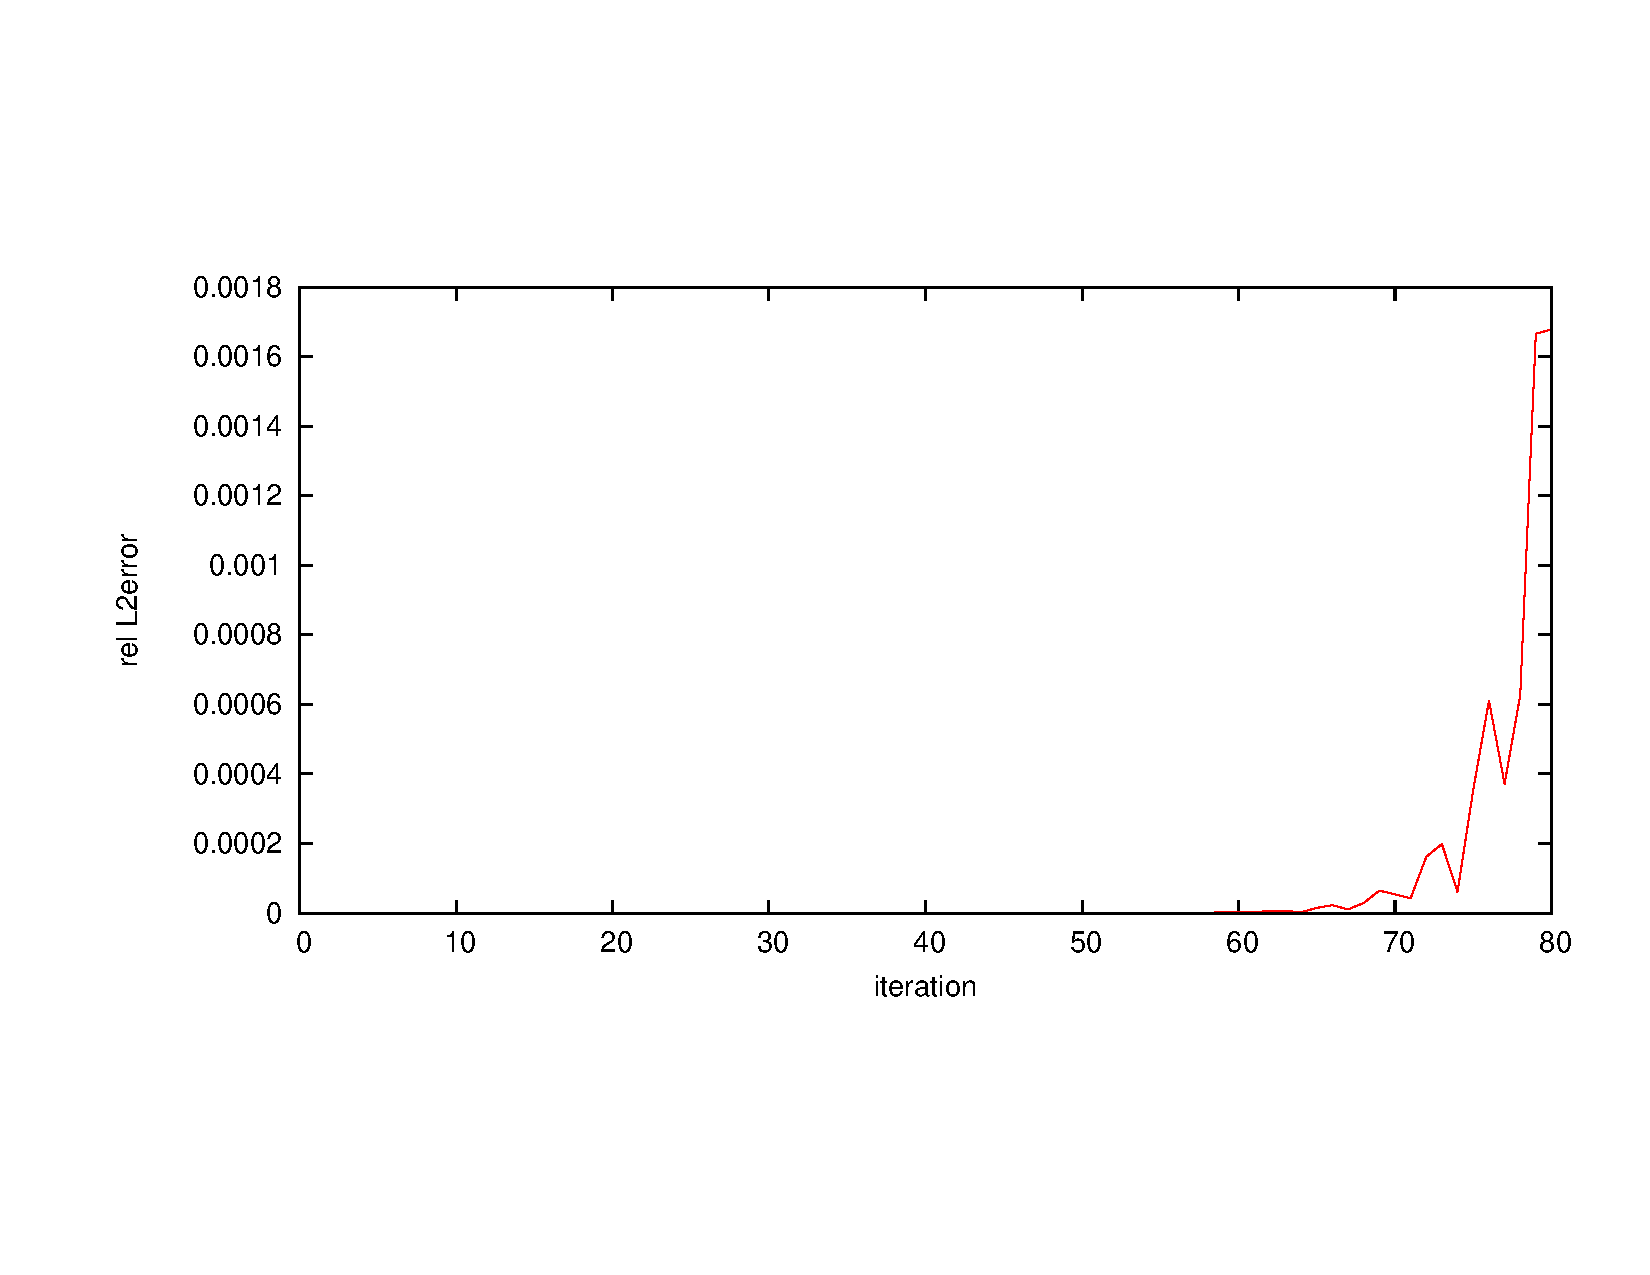
\includegraphics[trim = 2cm 4cm 1cm 4cm, scale =0.3]{../Arbeit/plots/consisctency_first_try.pdf}
	\caption{Relative $L^2$ error on a uniform grid with $h=\frac 1 2$}
	%\label{fig: consisctency_first_try}
\end{figure}
\end{frame}

\begin{frame}{An additional Penalty Parameter}
  \begin{columns}
	\begin{column}{0.9\textwidth}
%	\begin{wrapfigure}{r}{0.5\textwidth}
		\begin{figure}[H]
			\centering
%			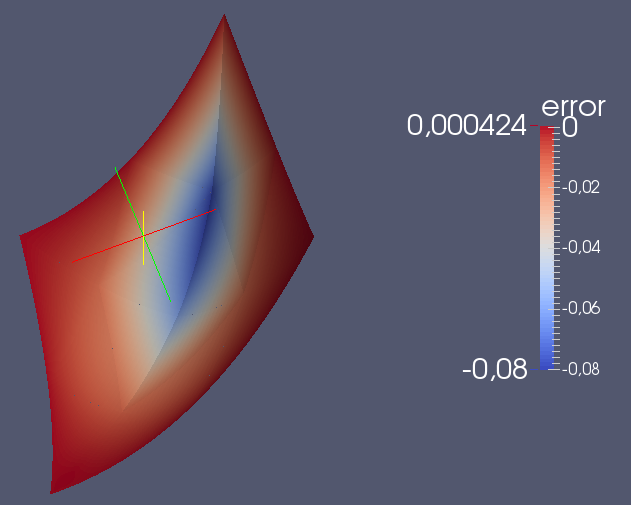
\includegraphics[width=.7\textwidth]{../Arbeit/plots/sharp_edges.png}
			\includemovie[ 
			 poster,controls, 
			 label=mylabel]{5cm}{5cm}{sharp_edges.u3d} 
			\caption{Numerical solution}
			\label{fig: sharp edges}
%	\end{wrapfigure}
		\end{figure}
	\end{column}
	\hspace{-1cm}
	\begin{column}{0.4\textwidth}
%		\todo{.vtu file?}
		\begin{itemize}
			\item sharp edges
			\item depends on triangulation
		\end{itemize}
	\end{column}
  \end{columns}
\end{frame}

\begin{frame}{An additional Penalty Parameter}
\begin{itemize}
\item force more regularity on the first derivative
\item Neilan used a further penalty term for low degrees
\end{itemize}
\[
	\sum_{e \in \edgesi} \sigma_g |e |\myIntS e {\jump{ \nabla u} \jump {\nabla v}}
\]

\vspace{1cm}
$\Rightarrow$ new method passes previous consistency test (with $\sigma_g$ =50)
\end{frame}

\begin{frame}{An additional Penalty Parameter}

	\begin{figure}[H]
	\begin{subfigure}[b]{.45\textwidth}
		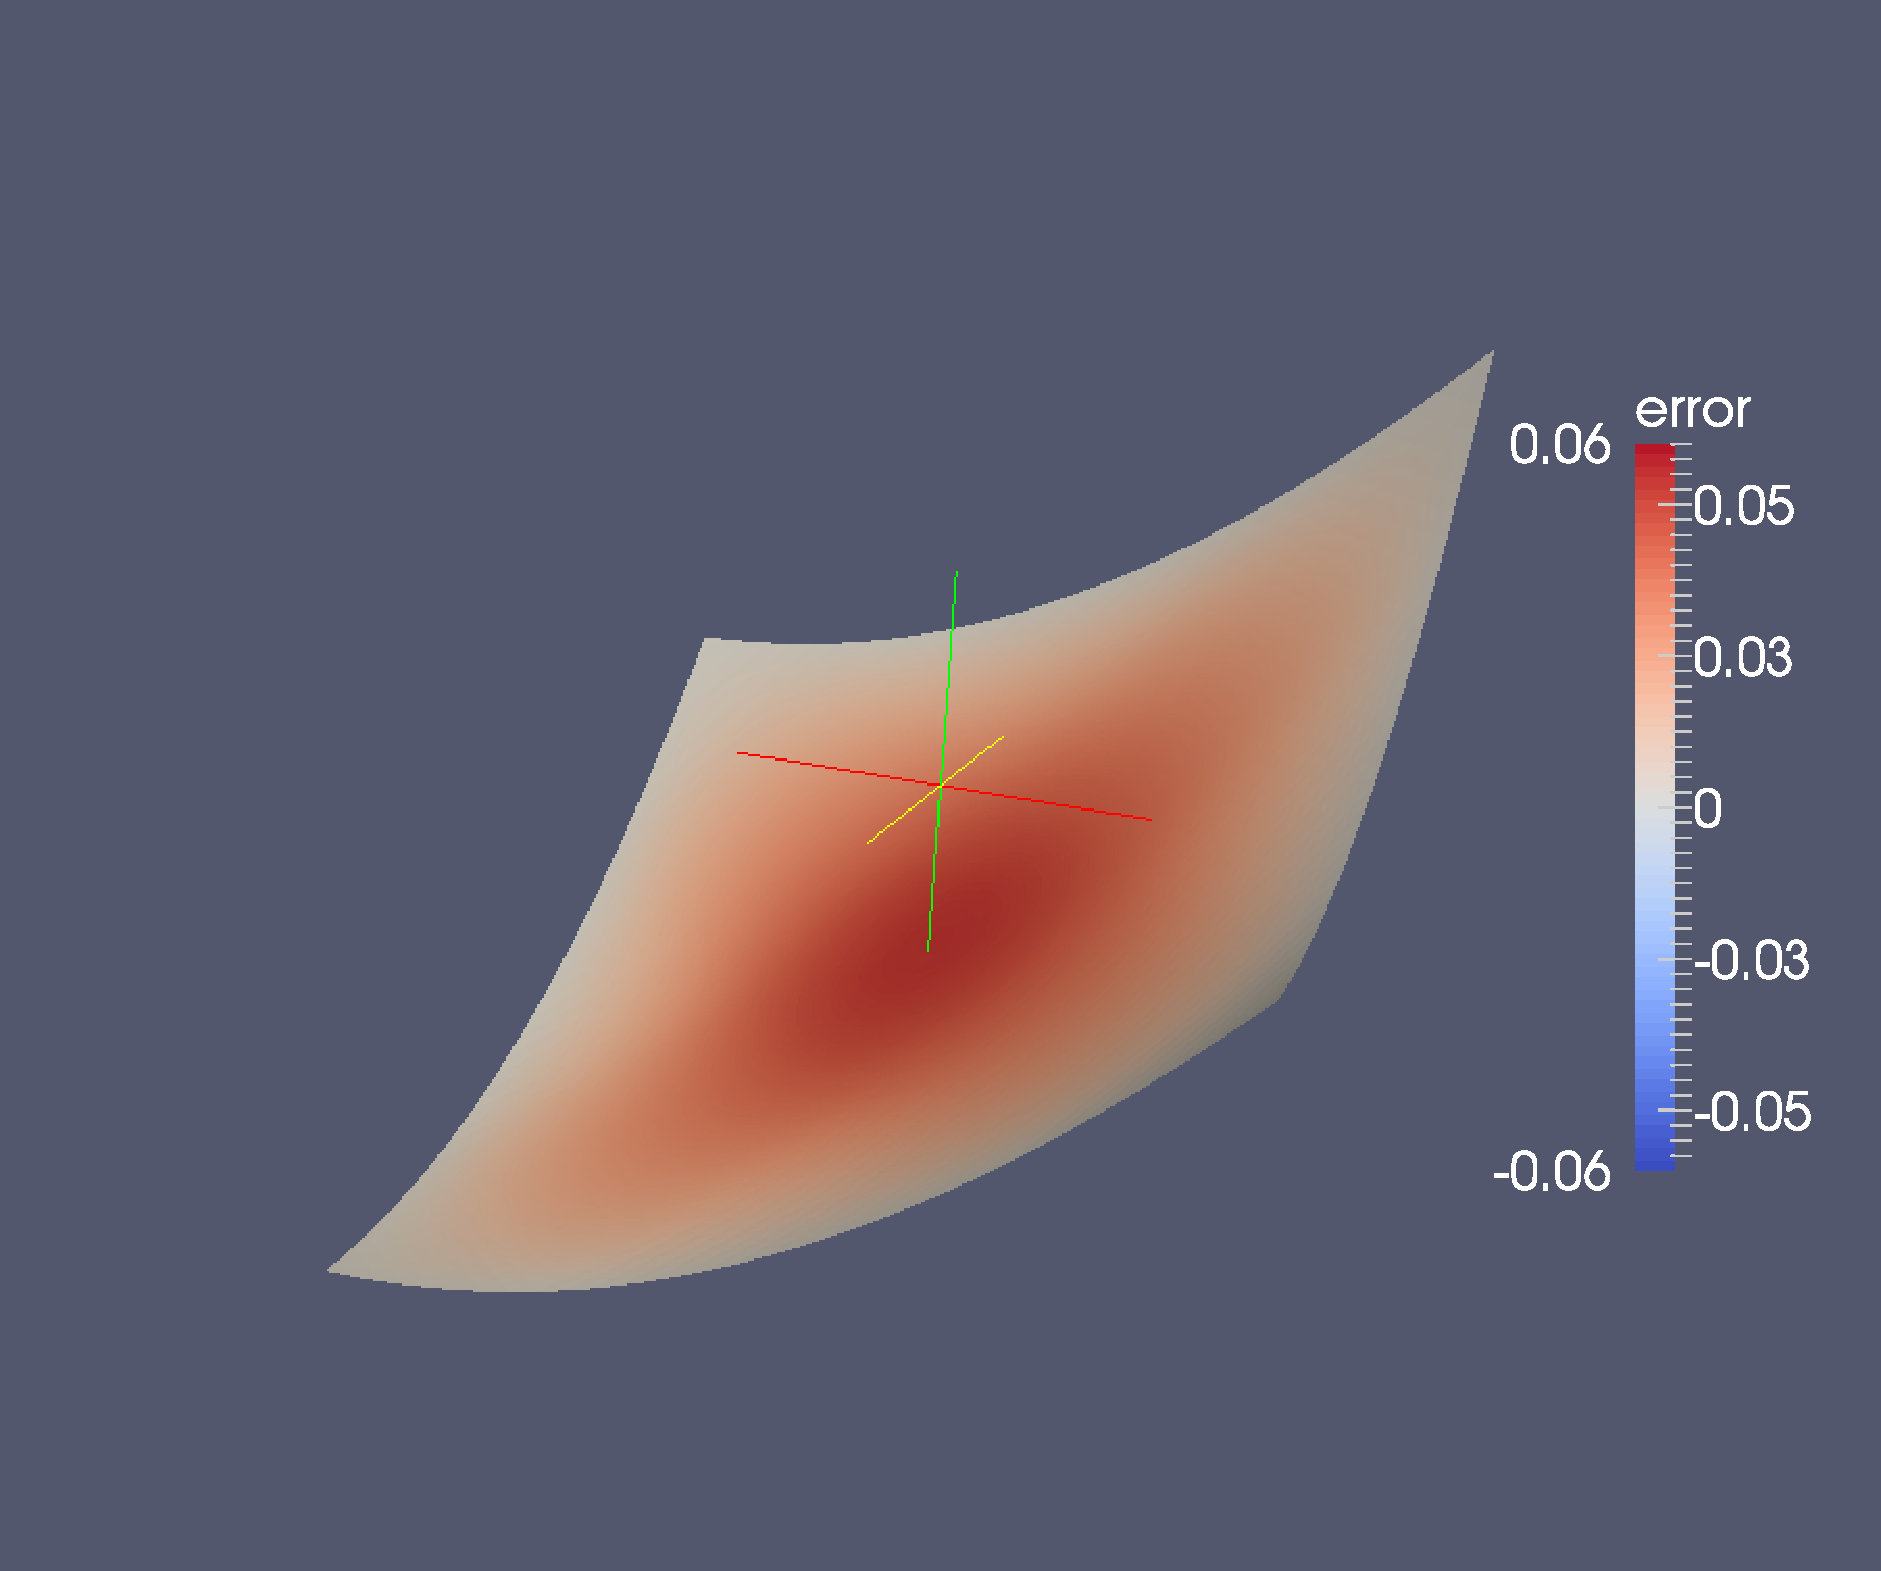
\includegraphics[width=1.\textwidth]{../Arbeit/plots/with_penalty_it22.pdf}
		\caption{Solution after 23 steps}
	\end{subfigure}
	~
	\begin{subfigure}[b]{.45\textwidth}
		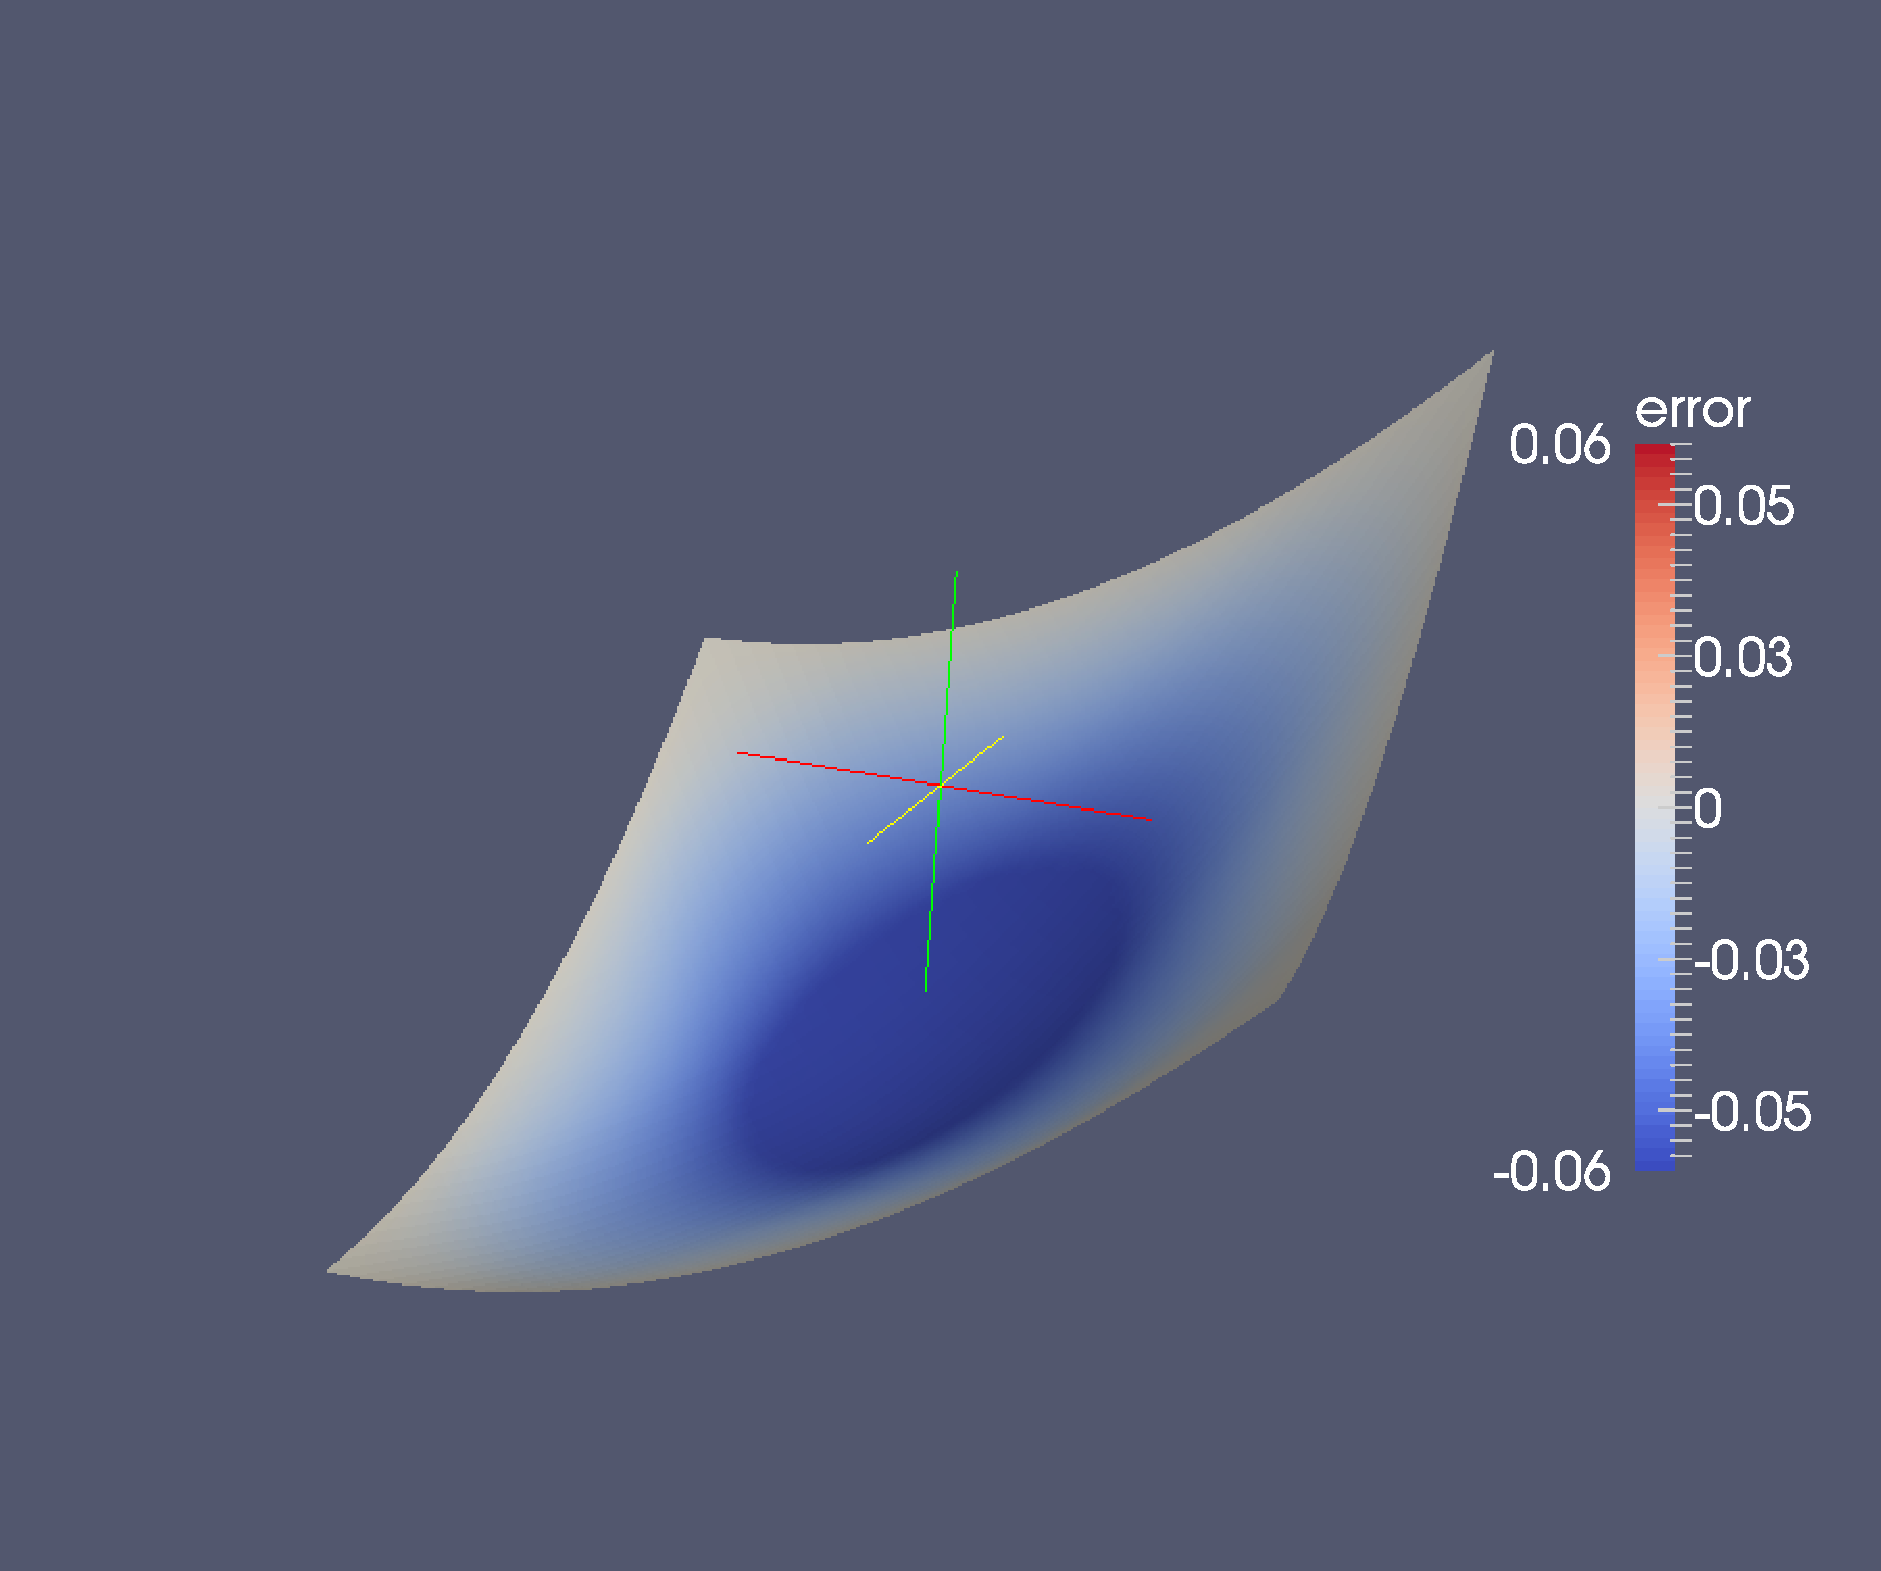
\includegraphics[width=1.\textwidth]{../Arbeit/plots/with_penalty_it23.pdf}
		\caption{Solution after 24 steps}
	\end{subfigure}
	\caption{The solution in two consecutive iterations}
	\end{figure}
\end{frame}

\begin{frame}{Damping}
	\begin{figure}[H]
		\centering
		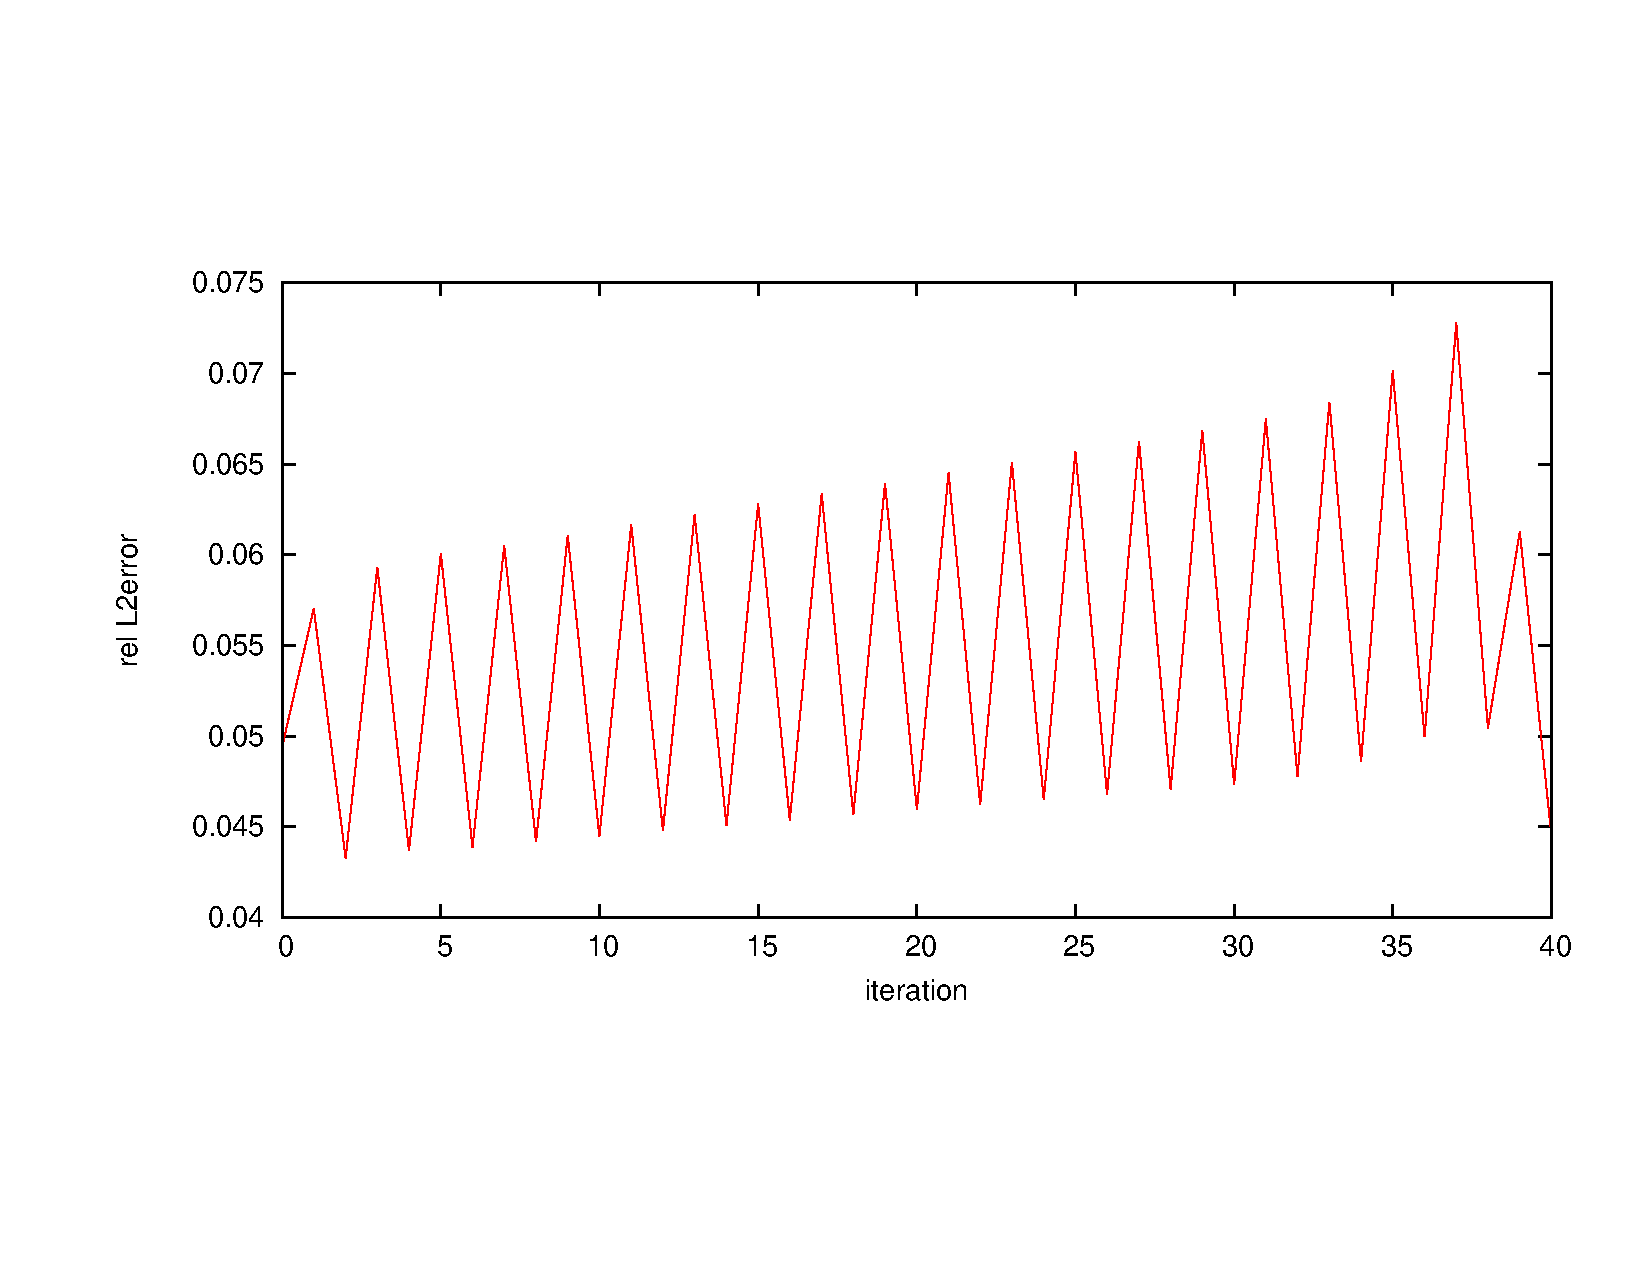
\includegraphics[trim = 2cm 4cm 1cm 4cm, height = 0.6\textheight]{../Arbeit/plots/oscillation.pdf}
		\caption{Relative $L^2$ error on a grid with $h=\frac 1 4$ and gradient penalty}
		\label{fig: oscillation}
	\end{figure}
	\pause
	\vspace{-0.5cm}
	$\Rightarrow$ Convex combination $ \alpha u_h^{i+1} + (1- \alpha) u_h^i$ for $\alpha \in (0,1)$
\end{frame}


\begin{frame}{Well-posedness of SIPG formulation}
\begin{itemize}
	\item The ellipticity constant of the SIPG bilinear form is only positive for $\sigma > \sigma^*$. 
	\pause
	
	\item $\sigma^*$ depends on $1/\lambda(\cofHess u)$, where  $\lambda(A)$ denotes the smallest eigenvalue of $A$.
\end{itemize}
	\pause
	$\Rightarrow$ scale $\sigma$ by $\frac 1 {\lambda^*}$ where $\lambda^*$ is an approximation of the smallest eigenvalue.\pause We choose
	
	\begin{block}{Approximation of $\lambda$}
	\[
		\lambda^* = \min_{q \in Q} \lambda(\cofHess {u_h(q)}),
	\]
	where $Q$ are the quadrature points.
	\end{block} 
	
\end{frame}

\begin{frame}{Well-posedness of SIPG formulation}
	For ellipticity of the SIPG bilinear form we need $\mycof {D^2_h u_h}$ to be positive definite.\\
	\pause
		\[
			\mycof {D^2_h u_h} \text{ pos. def.} \Leftrightarrow \hess u \text{ pos. def.} \onslide<3->\Leftrightarrow u_h \text{ is convex}
		\]
	\pause
	aim: ellipticity constant bounded below with a constant
	\pause
	\begin{block}{Modified Cofactor Matrix}
		\[ 
			\mycofMod {D^2_h u_h} = \begin{cases}
			\mycof {D^2_h u_h} & \lambda \geq \varepsilon	\\
			\mycof {D^2_h u_h}+ (-\lambda+\varepsilon) Id%\begin{pmatrix} -\lambda+\varepsilon & 0 \\ 0 & -\lambda+\varepsilon \end{pmatrix} 
			& else
			\end{cases}
		\]
	\end{block}
\end{frame}



\begin{frame}{Convexification}
\begin{itemize}
	\item \MA equation in general does not posses a unique solution
	\item often (unique) convex solution required
	\item convexify the solution after every step
	\item convexification is not simple
	\item connection between convexity and B\'ezier polynomials
\end{itemize} 
\end{frame}

\begin{frame}{Convexification Approach of Schumaker and Speleers{, \cite{SS2014}}}
	Given the solution of the generalised Poisson problem $u^{gp}_h$ we seek for a convex spline minimising the error at the B\'ezier control points, i.e. 
\begin{block}{Quadratic Program for Convexification}
Find the B\'ezier coefficients $c$ minimising
	\begin{align*}
			\lVert A c - b \rVert_2, \qquad \text{ such that } Cc \geq 0. %\label{eq: convex lsq}
	\end{align*}
\end{block}
\begin{itemize}
	\item $A$ is the matrix evaluating the piecewise polynomial at the B\'ezier control points
	\item $b$ are the function values of $u^{gp}_h$ at the B\'ezier control points
	\item  $C$ is the matrix containing the conditions ensuring convexity on the whole domain
\end{itemize}

\end{frame}


%\subsection{Algorithm for the Picard Iteration}

\begin{frame}
\begin{algorithm}[H]
\begin{algorithmic}
\Require triangulation \triang, desired mesh width $h$, maximal number of intermediate steps $i_{max}$
\State $u_0\gets $ solution of  $
	\triangle u = \sqrt{2f} \text{ in } \Omega $ with $
	u = g \text{ on }\partial \Omega$ %\Comment initialisation
\While {$h < H$}
	\State $i \gets 0$
	\While {$i < i_{max} $}
		\State $\sigma \gets \sigma /\lambda(\hess{u_h^{i-1}}) $
		\State $u_i \gets$ sol of generalised Poisson problem w. modified cofactor matrix
		\State (convexify)
		\State $u_i \gets \alpha u_{i-1} + (1-\alpha)u_i $ \Comment convex combination
		\State $i \gets i+1$
	\EndWhile
	\State $h, \triang \gets h/2, \triangFine$
\EndWhile
\end{algorithmic}
\caption{Picard Iteration Algorithm to Solve the MA Equation}
\label{alg: final}
\end{algorithm}
\end{frame}



\section {DG Methods}

\begin{frame}
Naive Ansatz:
\begin{align*}
	\myIntX {\Omega} {\mydet {D^2 u} v} = \myIntX \Omega {fv} \qquad \text{ for all test functions } v. %\label{eq: naiv ansatz}
\end{align*}

\begin{figure}[H]
			\begin{center}
		\usetikzlibrary{matrix}

\begin{tikzpicture}[scale =2]
  \matrix (m) [matrix of math nodes,row sep=3em,column sep=4em,minimum width=2em]
  {
     F[u]=0 & F_h[u] =0 \\
     L_u(w) =0 & L_{u,h}(w_h)=0 \\};
  \path[-stealth]
    (m-1-1) edge node [left] {linearise} (m-2-1)
            edge node [above] {discretise} (m-1-2)
    (m-2-1.east|-m-2-2) edge node [below] {discretise} (m-2-2)
    (m-1-2) edge node [right] {linearise} (m-2-2);
\end{tikzpicture}
		\end{center}

	\caption{An abstract diagram about the relation between weak and strong linear operators. The diagram is taken from \cite[Fig 2.2]{FGN2013}}
%		\label{fig: fe diagram}	
	\end{figure}
\end{frame}

\subsection{A $C^0$ Penalty Method }
\begin{frame}{A $C^0$ Penalty Method of Brenner et al.}
In \cite{BGN+2011} Brenner et alt. develop a method for $C^0$ elements
\pause

They add terms to the \quoting{naive ansatz} such that 
\begin{align*}
	\bilin {F (u+w)} v = \bilin {L_{u,h} w} v + \bilin {Rw} v,
\end{align*}
where $L_{u,h}$ is a stable and consistent discretisation of $L_u$.

\end{frame}

%\begin{frame}
%Let $V_h$ be ...
%\begin{block}{A $C^0$ penalty method for the MA problem }
%Find $u_h \in V_h$ such that
%\begin{align*}
%	&\myIntX {\Omega} {\left(f-\mydet {D^2_h u_h}\right) v_h} 
%	+ \sum_{e \in \edgesi} \myIntS e { \jump {\average{\mycof{D^2 u_h} } \nabla u_h} v_h} \\
%	&- \sum_{e \in \edgesb} \myIntS e { \jump{ \average{\mycof{D^2 u_h} } \nabla v_h} (u_h -g)} \\
%	&+ \sigma  \sum_{e \in \edgesb} \frac 1 {h_e} \myIntS e { (u_h -g)} \; = 0 \qquad \forall v_h \in V_h %\label{eq: brenner method}
%\end{align*}
%\end{block}
%\end{frame}

\subsection{A Finite Element Method based on a Discrete Hessian}

\def \boxContent {	The discrete Hessian $D_{DH}^2 u$ of $u$ is the unique function which satisfy for all $B \in \Sigma_h=[\mathcal{P}_h^k]^{d \times d}$
		\begin{align*}
			\myIntX  \Omega { (D_{DH}^2 u : B) }
			= \myIntX  \Omega { D^2_h u: B}
				 -\sum_{ e \in \edgesi} \myIntS e {  \jump {\average B \nabla u }}. %\label{eq: discrete hessian}
		\end{align*}}

\begin{frame}
The Hessian fulfils for all $B \in [H^1(\Omega)]^{d \times d}$
	\begin{align}
		\myIntX  \Omega { (D^2 u : B)} = 
			- \myIntX  \Omega { \left(\nabla \cdot B\right) \cdot \nabla u} 
			+ \myIntS {\partial \Omega}  {B \nabla u \; \mathbf {n}}, \label{eq: part int hessian}
	\end{align}
	\onslide<2->{ the piecewise Hessian in general not.}
\begin{overlayarea}{\textwidth}{0.7\textheight}
	\only<3>{
		\vspace{1cm}
		Idea by Lakkis and Pryer \cite{LP2011} and generalised by Neilan \cite{Neilan2014}: \\
		Replace Hessian by a discrete counterpart such that \eqref{eq: part int hessian} holds.		
	}
	\onslide<4->
	{
	\begin{block}{Definition of Discrete Hessian}
		\boxContent
	\end{block}
	}
	
	\onslide<5-> {Note that in general the discrete Hessian is not symmetric.}
	\end{overlayarea}
\end{frame}

\begin{frame}
\begin{block}{A FE Method based on a Discrete Hessian}
Find $u_h \in V_h$ such that
\begin{align*}
		\myIntX  \Omega { \left(\mydet{D_{DH}^2 u_h} - f \right) v_h} = 0 \qquad \forall v_h \in V_h, %\label{eq: neilan eq1}
\end{align*}
where $D_{DH}^2 u_h$ satisfies for all $B_h \in \Sigma_h$
	\begin{align*}
		\myIntX  \Omega { (D_{DH}^2 u_h : B_h) }
		= \myIntX  \Omega { D^2_h u_h: B_h}
			 -\sum_{ e \in \edgesi} \myIntS e {  \jump {\average {B_h} \nabla u_h }}. %\tag{\ref{eq: discrete hessian}}
	\end{align*}
\end{block}
\end{frame}

\begin{frame}
Special case for polynomial degree $k=1$

\begin{block}{A FE Method based on a Discrete Hessian}
Find $u_h$ in $V_h$ such that for all $v \in V_h$
\begin{align*}
		\myIntX  \Omega { \left(\mydet{D_{DH}^2 u_h} - f \right) v_h}+ \textcolor{red}{\sum_{e \in \edgesi} \sigma |e |\myIntS e {\jump{ \nabla u} \jump {\nabla v}}} = 0, %\label{eq: neilan eq1}
\end{align*}
where $D_{DH}^2 u_h$ satisfies for all $B_h \in \Sigma_h$
	\begin{align*}
		\myIntX  \Omega { (D_{DH}^2 u_h : B_h) }
		= \myIntX  \Omega { D^2_h u_h: B_h}
			 -\sum_{ e \in \edgesi} \myIntS e {  \jump {\average {B_h} \nabla u_h }}. %\tag{\ref{eq: discrete hessian}}
	\end{align*}
\end{block}
\end{frame}


\section{Numerical Results}

\subsection{A $C^0$ Penalty Method}
\begin{frame}{Implementation}
	\begin{itemize}
		\item implemented with finite element tool FEniCS
		\item nested iteration with initial guess $\triangle u = - \sqrt{2f}$
		\item uniform standard refinement
		\item nonlinear system solved PETSc with FEniCS default configuration: a Newton based nonlinear solver using a basic line search, arising linear systems are solved by a $LU$ decomposition.
		\item absolute tolerance is adjusted to $1e-8$ and number of maximum iteration restricted to 100
	\end{itemize}
\end{frame}

\begin{frame} %{Smooth Test Case}
%\begin{block}
Smooth Test Problem:
\[
	u=\exp( \lVert x \rVert_2^2  /2) 
	\text { and } 
	f = (1 + \lVert x \rVert_2^2) \exp( \lVert x \rVert^2).
\]
%\end{block}
\vspace{-1cm}
\begin{figure}[H]
\centering
	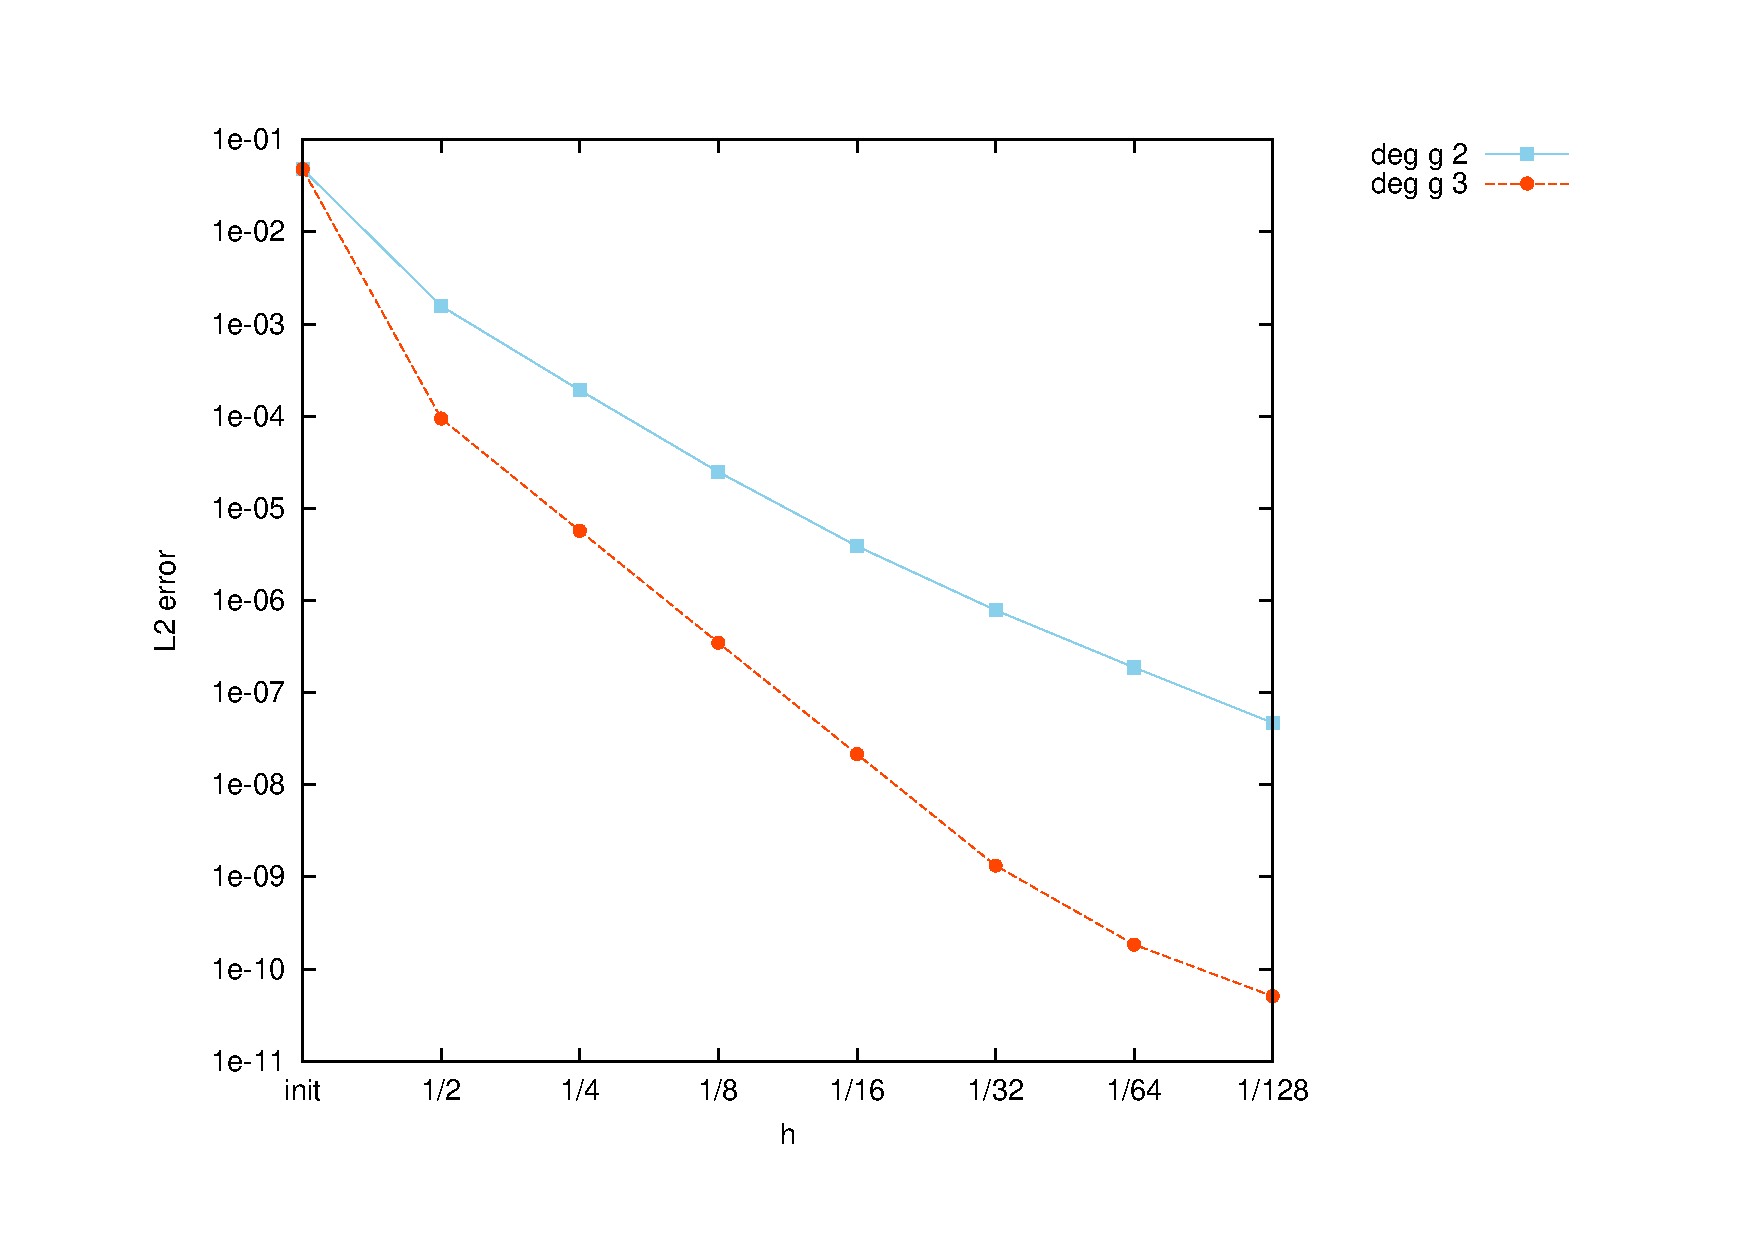
\includegraphics[width=0.95\textwidth]{../Arbeit/plots/MA1_Brenner_l2.pdf}
	\caption{$L^2$ errors for the smooth test case}
	\label{fig: Brenner test1}
\end{figure}
\end{frame}

%\newcommand{\readData}[2]{
%	\pgfplotstableread{../Arbeit/data/#1_l2errornorm} #2
%	
%	\pgfplotstablecreatecol[copy column from table={../Arbeit/data/#1_h1errornorm}{h1error}] {h1error} #2
%	
%	\pgfplotstablecreatecol[copy column from table={../Arbeit/data/#1_newtonSteps}{steps}] {N} #2
%}

%\readData{MA3_Brenner_deg2}{\MAThreeBrennerTwo}
%\readData{MA3_Brenner_deg3}{\MAThreeBrennerThree}

%\begin{frame}
%
%\begin{table}[h]
%\centering
%	\begin{subtable}[b]{0.45\textwidth}
%		\centering
%		\pgfplotstabletypeset[columns={iterations, l2error, h1error,N},
%				    every row 0 column 0/.style={set content=init},
%		]\MAThreeBrennerTwo
%    	\caption{Error for $k=2$}
%    \end{subtable}
%   ~
%	\begin{subtable}[b]{0.45\textwidth}
%		\centering
%		\pgfplotstabletypeset[columns={iterations, l2error, h1error,N},
%				    every row 0 column 0/.style={set content=init},
%				    every row 0 column 0/.style={set content=init},
%				    every row 3 column 1/.style={set content=-},
%				    every row 3 column 2/.style={set content=-},
%				    every row 3 column 3/.style={set content=-},
%				    every row 4 column 1/.style={set content=-},
%				    every row 4 column 2/.style={set content=-},
%				    every row 4 column 3/.style={set content=-},
%		]\MAThreeBrennerThree
%    	\caption{Error for $k=3$}
%    \end{subtable}	\caption{Errors for Test \ref{test singularity}}
%	\label{tab: l2 errors test 3 Brenner}
%\end{table}
%\end{frame}

\subsection{A FE Method based on the Discrete Hessian}

\begin{frame} %{Smooth Test Case}
Smooth Test Problem:
\[
	u=\exp( \lVert x \rVert_2^2  /2) 
	\text { and } 
	f = (1 + \lVert x \rVert_2^2) \exp( \lVert x \rVert^2).
\]
\vspace{-1cm}
\begin{figure}[H]
\centering
	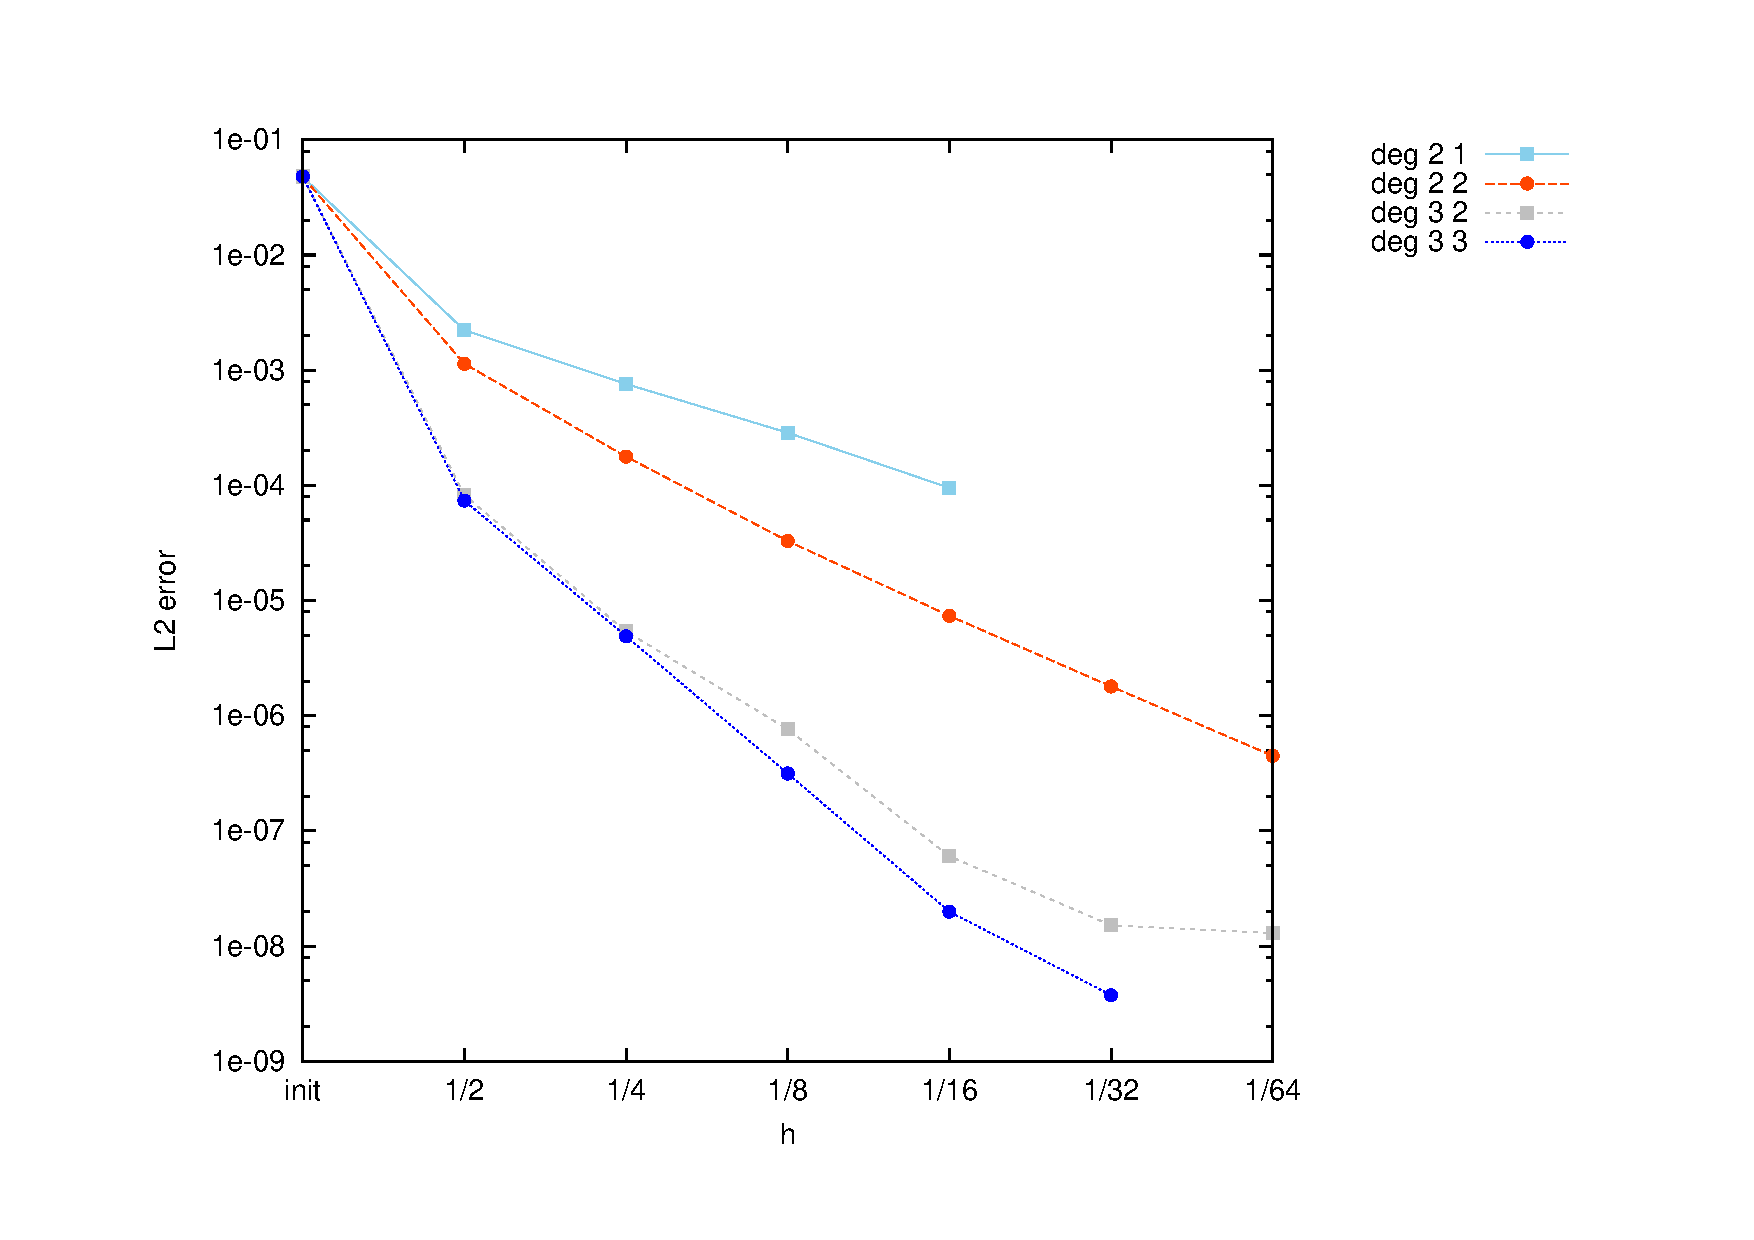
\includegraphics[width=0.95\textwidth]{../Arbeit/plots/MA1_Neilan_l2.pdf}
%	\caption{$L^2$ errors for Test \ref{test smooth}}
\end{figure}
\end{frame}

\begin{frame}
Smooth Problem solved with additional gradient penalty
\vspace{-.75cm}
	\begin{figure}[H]
	\centering
	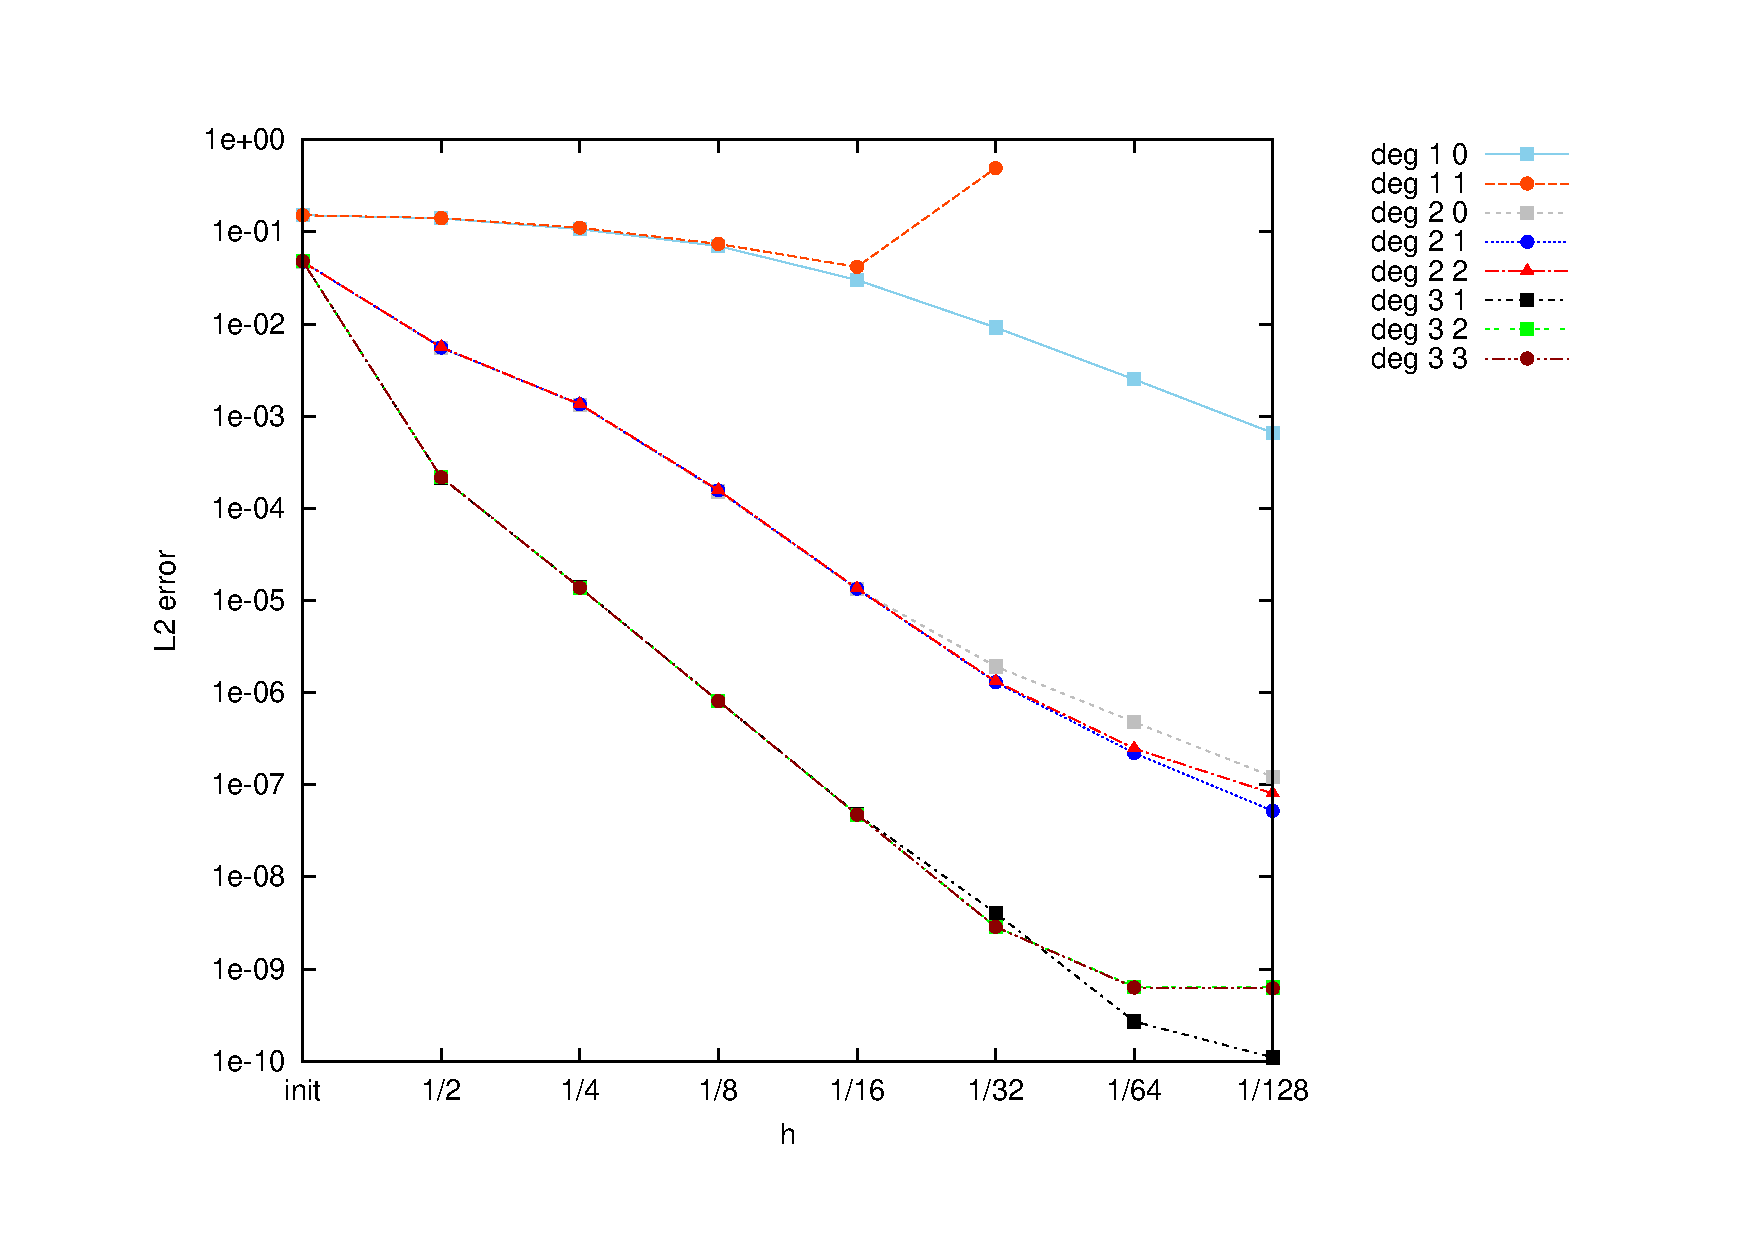
\includegraphics[ %trim = 3cm 4cm 0cm 2cm,
	width=\textwidth]{../Arbeit/plots/MA1_Neilan_GradJump_l2.pdf}
%		\caption{$L^2$ error with grad penalty}
	\end{figure}
\end{frame}

\begin{frame}
Smooth Problem solved with additional gradient penalty
\vspace{-.75cm}
	\begin{figure}[H]
	\centering
	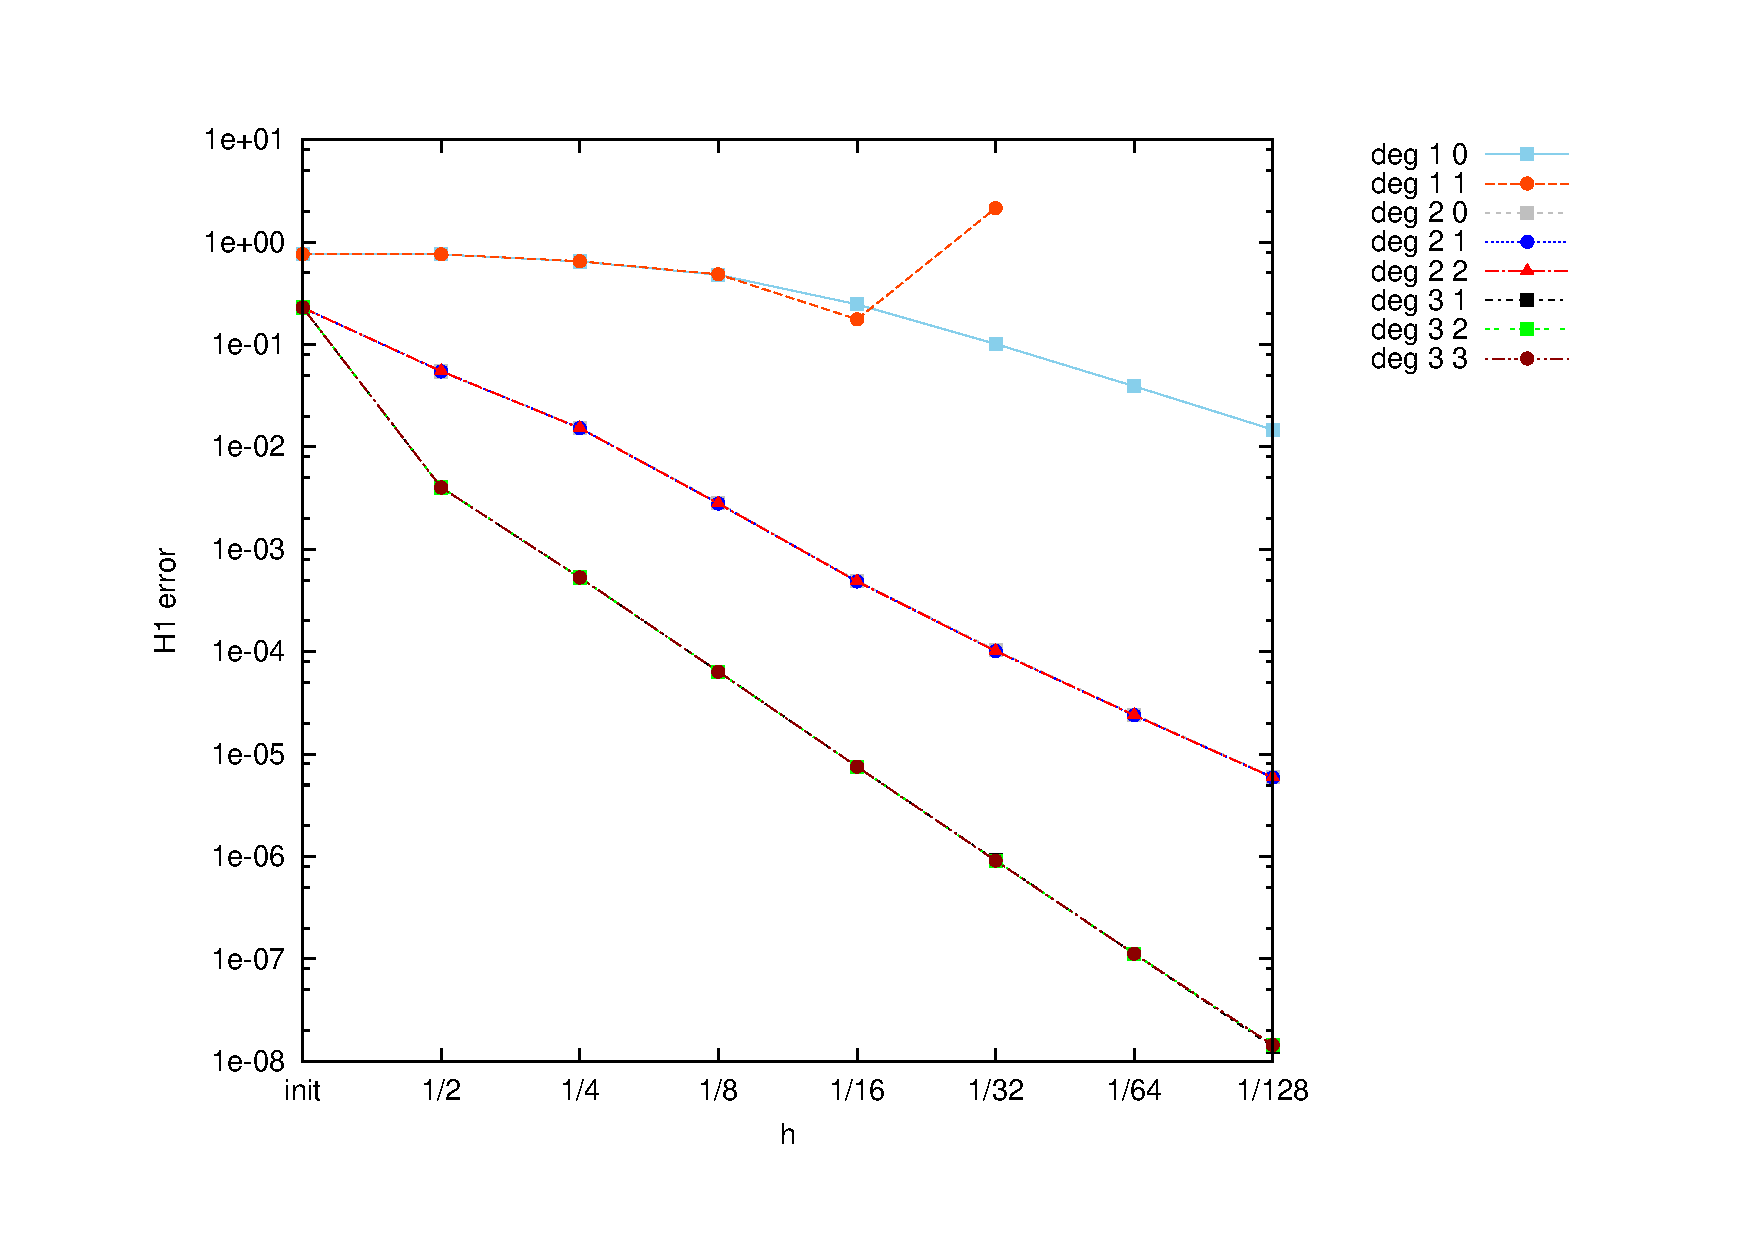
\includegraphics[ %trim = 3cm 4cm 0cm 2cm,
	width=\textwidth]{../Arbeit/plots/MA1_Neilan_GradJump_h1.pdf}
%		\caption{$L^2$ error with grad penalty}
	\end{figure}
\end{frame}

\subsection{Picard Iteration}
\begin{frame}
Smooth Problem solved with Picard Iteration
\vspace{-.75cm}
	\begin{figure}[H]
	\centering
	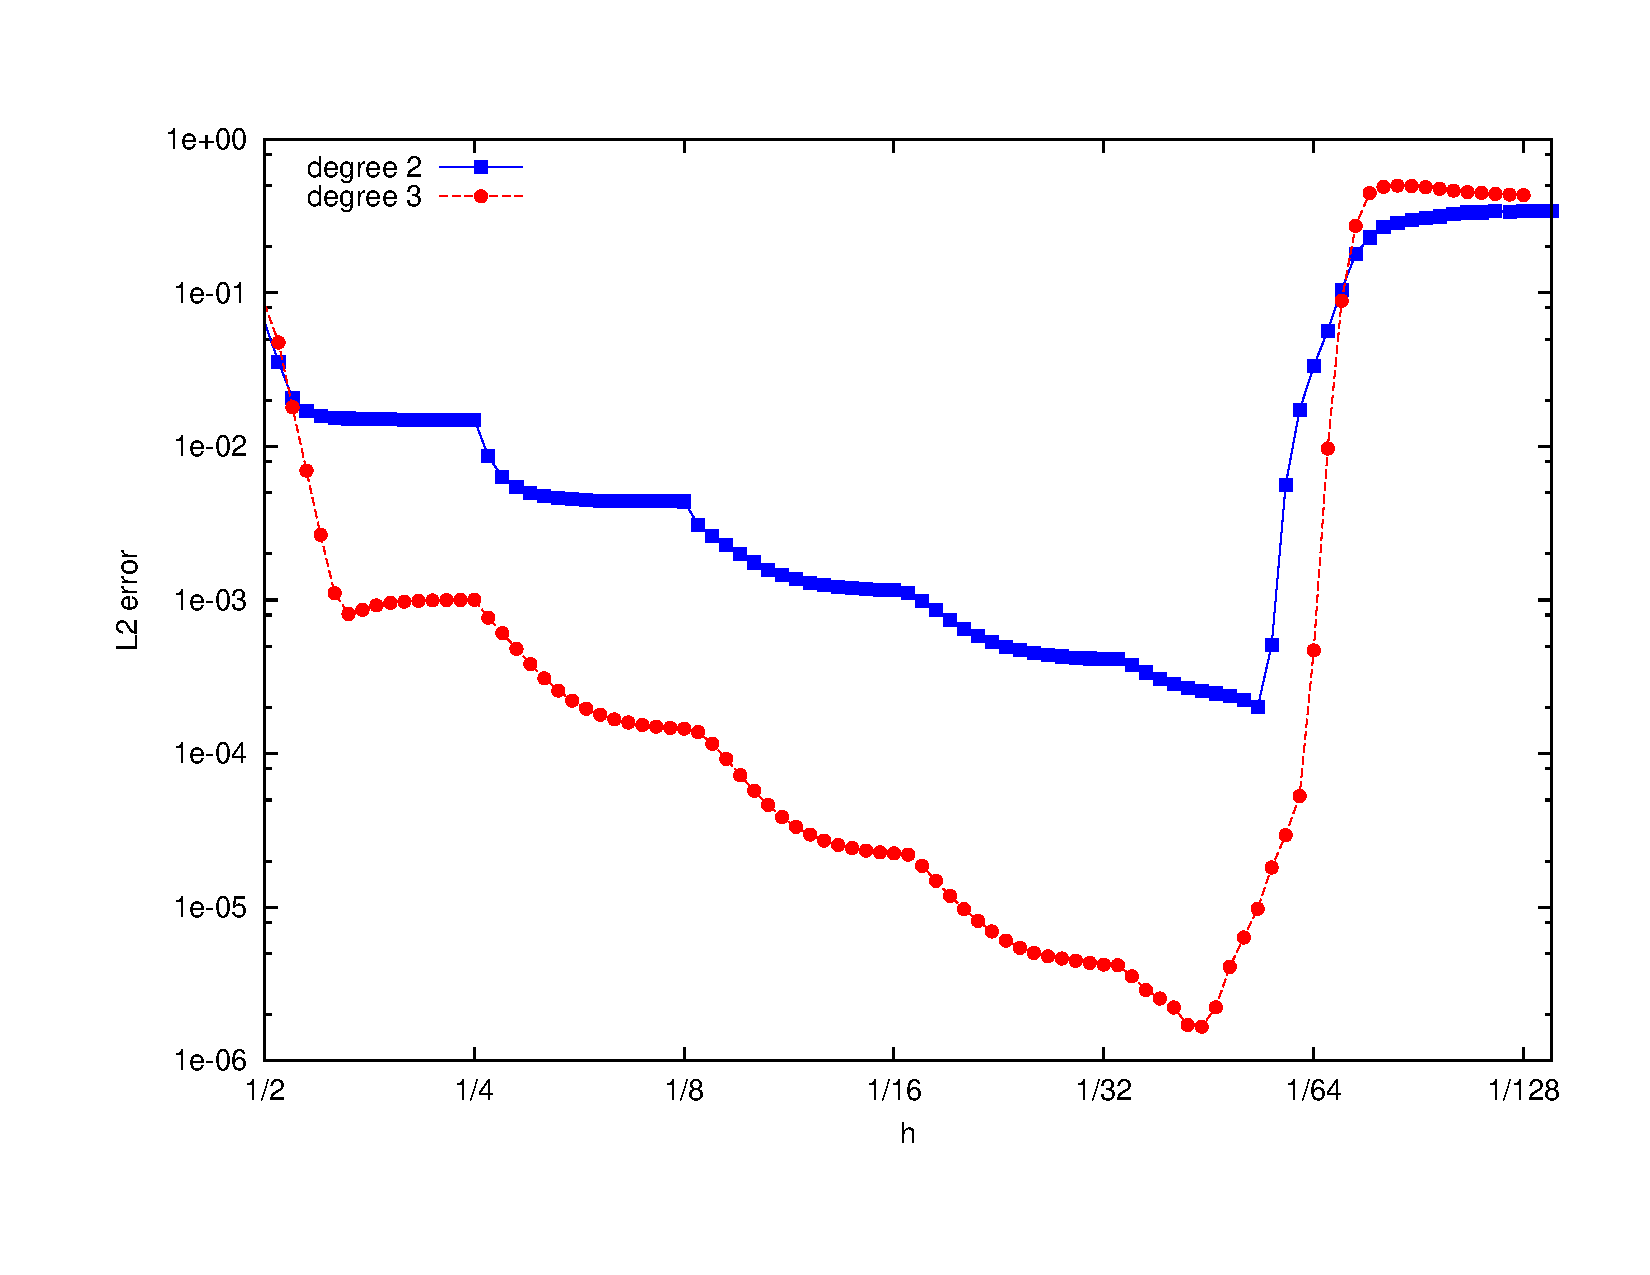
\includegraphics[ %trim = 3cm 4cm 0cm 2cm,
	width=\textwidth]{../Arbeit/plots/MA1.pdf}
%		\caption{$L^2$ error with grad penalty}
	\end{figure}
\end{frame}


\section{Conclusion and Perspective}

\begin{frame}{Conclusion}
	\begin{itemize}
		\item derived a new DG using Picard linearisation
		\item the $C^0$ penalty method developed by Brenner et al. yields good results for smooth cases, but fails in non-smooth cases
		\item the method based on a discrete Hessian improved by Neilan converges in smooth cases as well as in non-smooth tests
		\item the Picard type iteration converges on coarse grids, but is unstable on finer grids
		\item Neilan's method requires a lot of degrees of freedom
		\item current DG methods are applicable for problems with smooth solutions
	\end{itemize}
\end{frame}

%\subsection{Conclusion}
	
\begin{frame}{Perspective}
	\begin{itemize}
		\item decoupled PDE has more solutions than the solution $v=w$
		\item apply theory developed for Picard linearisations of convection terms
		\item implemented convexification not useful, may only convexify on finer grids
		\item extension to right-hand sides depending on $u$ and $\nabla u$ and more complicated left-hand sides
		\item three-dimensional case
		\item analysis of the impact of the gradient penalty term
	\end{itemize}
\end{frame}


%\subsection{Perspective}

\begin{frame}[allowframebreaks]{References}
\bibliography{../Arbeit/my_additional_bibliography.bib}
\bibliographystyle{plain}
\end{frame}

\end{document}